\scanpage{188}
% L01–04
L'\deleted{\unsure{entier}}\inserted{élément} $\gamma$ dépend a priori du choix de $s$, Mais \deleted{\unsure{si $s$|si on}} par transport de structure, on voit qu'il est le $=$ pour $s$ et \inserted{pour} $us$, $u\in G_0$, donc que il est en fait indépendant de $s$.

% L05–09
Mais \deleted{cela montre que l'on a} \inserted{on voit alors que} la structure $A_\lambda$ est entièrement déterminée par \deleted{\unsure{l'entier|l'indice}} l'élément
\[
\gamma\in Z'_n=(\mathbb Z/n\mathbb Z)^{\unsure{*|d}}/\pm1\tag*{(28)}
\]
puisque l'on a
\[
A_\lambda=\bigcup_{\substack{E\in{\unsure{\mathscr E|\mathcal E|\Sigma}}^{\unsure{a|0}}\\\text{ens des étoiles de } S\\(\text{le }=\text{ pour }A_0\text{ et }A_\lambda}}
\bigl(A_{E,\lambda}=A_{E,\unsure{0|.}}^{(\gamma)}\bigr).\tag*{(29)}
\]

% L10–16
Cet argument marche si, au lieu de supposer l'homothétie stricte, on suppose la chose suivante
\[
\deleted{\unsure{\mathrm P_2}}\left\{\begin{aligned}
\text{b)}\ &\text{Toute étoile }\inserted{E}\text{ est, }\deleted{\unsure{E}}\text{ pour la structure}\\
&A_{\lambda E}=A_\lambda\cap\unsure{\mathfrak P_2(E)|\mathrm P_2(E)},\ \text{un polygône}\\
&\text{combinatoire}\\
\text{a)}\ &\text{Toute }a\in A_\lambda\text{ est contenue dans}\\
&\text{au moins une étoile}
\end{aligned}\right.\tag*{(30)}
\]
% Curved transposition arrow from b) pointing below a).
\noindent\smash{\raisebox{1.3ex}{\begin{tikzpicture}[overlay]\draw[->] (0,1.4) to[bend right=30] (.26,0);\end{tikzpicture}}}

% L17–22
Notons que le groupe $G_0$ opère par automorphismes de $A_\lambda$, et qu'il opère transitivement sur l'ens des arêtes orientées de $G_0$. Il en résulte que \inserted{il suffit de vérifier} les conditions a) b) pour \uline{une} étoile $E$, pour \uline{une} arête $a$. \deleted{\unsure{de}} Pour la condition a) il suffit de prouver donc

% archive sheet number: 187
